\documentclass{article}
\usepackage{enumitem}
\usepackage{graphicx}
\usepackage[style=ieee,backend=biber]{biblatex}
\usepackage{hyperref}
\usepackage{amsmath}
\usepackage{listings}
\usepackage{xcolor}
\usepackage{float}

\addbibresource{externe.bib}

\title{Milestone 1: Transport Station Live Feed}
\author{Graf Cem IM7}
\date{June 2025}

\begin{document}

\maketitle

\tableofcontents
\clearpage

\section{Overview}
In this project, I want to process the live feed of a transportation provider and answer the following questions:
\begin{enumerate}
    \item Given the current location of a person and number $K$ as input, find the $K$ nearest stations with available devices such as bikes or scooters.
    \item Given the current location of a person who has a bike or scooter and number $K$ as input, find the $K$ nearest stations where docks are available.
    \item Given a source and destination location (e.g., Los Angeles), present the route using Metro Bike on a mapping product such as Google Maps.
\end{enumerate}

\section{Source}
The source was retrieved from \url{https://bikeshare.metro.net/about/data/}.

\section{Tools}
\begin{itemize}
  \item Python
  \item Visual Studio Code
  \item Docker
  \item Git
  \item PostgreSQL + PostGIS (GiST R-Tree)
  \item Streamlit
  \item pytest
\end{itemize}

\section{First Approach -- Core Assumptions \& Baseline Algorithms}

\subsection{Data Pipelines (Crawler \& Extract, Transform, Load)}
\begin{enumerate}[label=3.1.\arabic*]
  \item \textbf{Static-Station Crawler (monthly):} fetch \texttt{station\_information.json}, process and store station updates in the database and spatial index, and record any schema changes.
  \item \textbf{Live-Status Crawler (every 60\,s):} periodically retrieve station status updates and store them in the database.
  \item \textbf{Trip-CSV Ingest (quarterly):} load and cleanse trip CSVs.
  \item \textbf{Station Master SCD (on update):} detect and record changes in station metadata.
\end{enumerate}

\subsection{Spatial Index}
Store station coordinates as \texttt{GEOGRAPHY(Point)} with a GiST (R-Tree) index for efficient nearest-neighbor searches combined with attribute filters.

\subsection{Sparse k-NN Station Graph}
\begin{itemize}
  \item Connect each station to its $k \approx 5\text{--}8$ nearest neighbors, yielding $O(k\cdot |V|)$ edges.
  \item Edge attributes begin as simple distance estimates and are later replaced by realistic ETAs, sourced either from OpenRouteService \textbf{or} median trip durations from trip data.
\end{itemize}

\subsection{Task Workflows}
\begin{itemize}
  \item \textbf{Task 1 -- $K$ nearest stations with devices:} insert a virtual \texttt{USR} node, query the $k$ nearest via the R-tree, filter stations where \texttt{num\_bikes\_available + num\_ebikes\_available + num\_scooter\_available > 0}, and increase $k$ until at least $K$ valid results are found.
  \item \textbf{Task 2 -- $K$ nearest stations with free docks:} same flow as above, but filter on \texttt{num\_docks\_available > 0}.
  \item \textbf{Task 3 -- Routing SRC $\to$ DST:} insert \texttt{SRC} and \texttt{DST} nodes; connect \texttt{SRC} to its $k$ nearest stations via walking edges (if devices are available) and connect stations near \texttt{DST} via walking edges (if docks are available). Compute the shortest path with Dijkstra or A*.
\end{itemize}

\section{Milestone 1}

\subsection{Scraper Workflow}
The entry point \texttt{scraper.py} takes a data type (\textit{trip}, \textit{station} or \textit{geojson}) and a destination directory.
\begin{itemize}
    \item \texttt{--interval 0}: one-time run (cron job)
    \item \texttt{--interval >0}: continuous worker (Docker service)
\end{itemize}
Each scraper module handles its own download and cleaning flow, isolating schema changes.

\begin{figure}[H]
    \centering
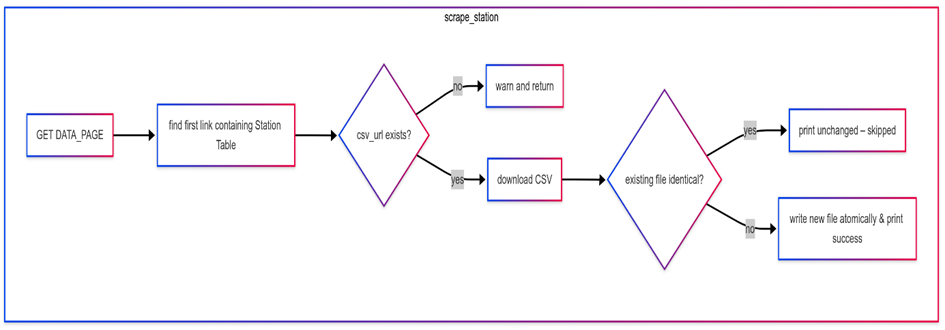
\includegraphics[width=0.8\textwidth]{stionScraper.png}
    \caption{Station table scraping workflow}
    \label{fig:flowchart_station}
\end{figure}

\begin{figure}[H]
    \centering
   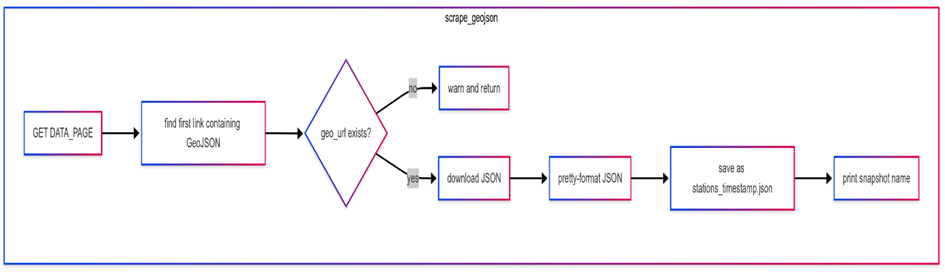
\includegraphics[width=0.8\textwidth]{geojsonScraper.png}
    \caption{GeoJSON live feed scraping workflow}
    \label{fig:flowchart_geojson}
\end{figure}

\begin{figure}[H]
    \centering
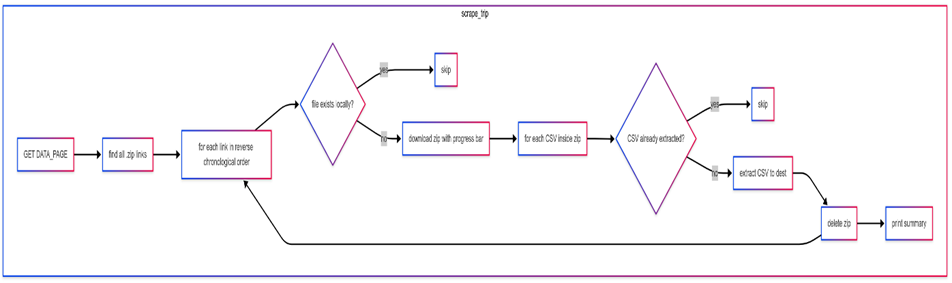
\includegraphics[width=0.8\textwidth]{tripScraping.png}
    \caption{Trip data scraping workflow}
    \label{fig:flowchart_trip}
\end{figure}

\section{Data Acquisition}

\subsection{\texttt{scraper.py} Excerpt}
\begin{lstlisting}[language=Python]
class Kind(Enum):
    trip = "trip"
    station = "station"
    geojson = "geojson"

    DATA_PAGE = "https://bikeshare.metro.net/about/data/"
    STATION_URL = "https://bikeshare.metro.net/static/station_table.csv"
    GEOJSON_URL = "https://bikeshare.metro.net/stations/stations.geojson"
\end{lstlisting}

Usage examples:
\begin{lstlisting}[language=bash]
# Monthly trip archive
python src/scraper/scraper.py -k trip -d ./scraper_data/trip_data -i 2628000

# On-demand station table
python src/scraper/scraper.py -k station -d ./scraper_data/static

# Live status every minute
python src/scraper/scraper.py -k geojson -d ./scraper_data/live -i 60
\end{lstlisting}

\section{Exploratory Data Analysis \& Quality}

\subsection{Null-value Distribution}

\begin{figure}[H]
    \centering
    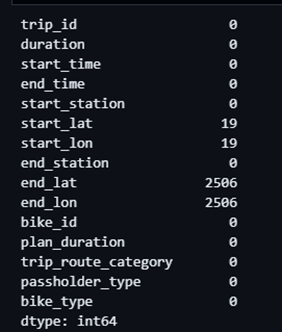
\includegraphics[width=0.8\textwidth]{tripdata.png}
    \caption{Null values chart for Trip data Q1~2025 (95\,916 rows)}
    \label{fig:null_values_trip_q1_2025}
\end{figure}

\begin{figure}[H]
    \centering
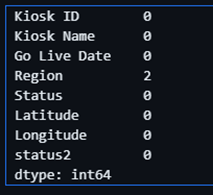
\includegraphics[width=0.8\textwidth]{stationdata.png}
    \caption{Null values chart for Station data April~2025 (221 rows)}
    \label{fig:null_values_station_apr_2025}
\end{figure}

\subsection{Cleaning Strategy}
Trip data:
\begin{table}[H]
\centering
\begin{tabular}{l l}
Field & Imputation / Action \\
 duration & Compute end\_time -- start\_time; else drop row \\
 start\_time & Compute end\_time -- duration; else drop row \\
 end\_time & Compute start\_time + duration; else drop row \\
 start\_lat/lon/station & Lookup in StationInfo; else drop row \\
 end\_lat/lon/station & Same as start fields \\
 bike\_type & Label as ``unknown\_device'' \\
\end{tabular}
\end{table}

StationInfo data:
\begin{table}[H]
\centering
\begin{tabular}{l l}
Field & Imputation / Action \\
 Station ID & Merge duplicates (incl. virtual station) \\
 Region & Label as ``Unknown'' or use reverse geocoding \\
 Station Name & Label as ``Unnamed Station'' \\
 Status & Label as ``Inactive'' or ``Unknown'' \\
\end{tabular}
\end{table}

\section{Persistence Layer}

\subsection{Docker Compose Excerpt}
\begin{lstlisting}[language=yaml]
services:
  db:
    image: postgis/postgis:15-3.3
    restart: unless-stopped
    environment:
      POSTGRES_USER: radverkehr
      POSTGRES_PASSWORD: passwort123
      POSTGRES_DB: radstationen
    volumes:
      - pgdata:/var/lib/postgresql/data
      - ./initdb:/docker-entrypoint-initdb.d
      - ./data:/data
    ports:
      - "5432:5432"
\end{lstlisting}

\section{Prototype SQL Queries}

\subsection{$K$-nearest Stations with Bikes}
\begin{lstlisting}[language=SQL]
WITH user_location AS (
  SELECT ST_SetSRID(ST_MakePoint(%s, %s), 4326)::GEOGRAPHY AS geom
)
SELECT s.station_id, s.name, s.num_bikes, s.num_docks, s.online,
       ST_Distance(s.geom, u.geom) AS distance_m
FROM public.stations AS s
CROSS JOIN user_location AS u
WHERE s.num_bikes > 0 AND s.online = TRUE
ORDER BY s.geom <-> u.geom
LIMIT %s;
\end{lstlisting}

\subsection{$K$-nearest Stations with Free Docks}
\begin{lstlisting}[language=SQL]
WITH user_location AS (
  SELECT ST_SetSRID(ST_MakePoint(%s, %s), 4326)::GEOGRAPHY AS geom
)
SELECT s.station_id, s.name, s.num_bikes, s.num_docks, s.online,
       ST_Distance(s.geom, u.geom) AS distance_m
FROM public.stations AS s
CROSS JOIN user_location AS u
WHERE s.num_docks > 0 AND s.online = TRUE
ORDER BY s.geom <-> u.geom
LIMIT %s;
\end{lstlisting}

\section{User Interface}
The first UI iteration uses Streamlit and Folium.

\begin{figure}[H]
    \centering
    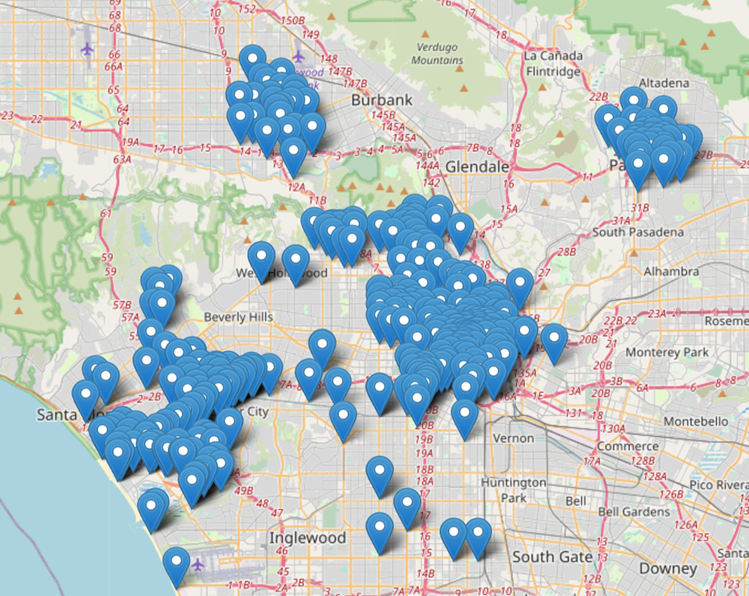
\includegraphics[width=0.8\textwidth]{FolioMap.png}
    \caption{Map showing all stations of the bike provider}
    \label{fig:map_all_stations}
\end{figure}

\section{Outlook}
\begin{itemize}
  \item Integrate OpenRouteService for Task~3 and extend the cost model (time).
  \item Implement dynamic $k$-NN edges and ML-based travel time estimation.
\end{itemize}

\section{Appendix}


\begin{figure}[H]
    \centering
 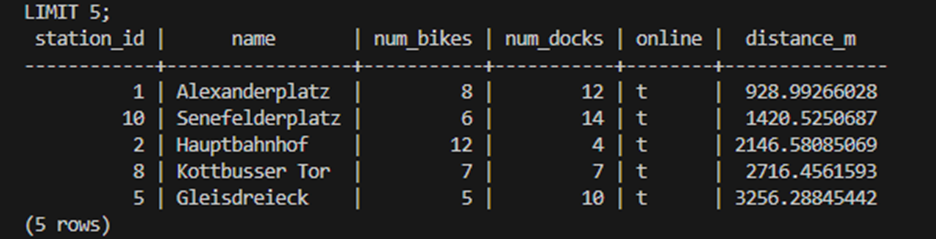
\includegraphics[width=0.8\textwidth]{test.png}
    \caption{Test of $K$-nearest station calculation}
    \label{fig:test_k_nearest}
\end{figure}

\printbibliography

\end{document}